\documentclass[a4paper]{article}

\usepackage{float}
\usepackage{graphicx}
\usepackage{hyperref}
\usepackage[all]{hypcap}

\title{Computer vision lab 1}
\author{Xeryus Stokkel (s2332795)}

\begin{document}

\maketitle

\section{Exercise 1}

The SIFT implementation returns a key array of dimensions $1021 \times 128$. We know that a SIFT feature vector can either have a size of 128 or 160 elements, so from this we can see that there are 1021 keys in total. From \cite{lowe1999object} we know that the algorithm generates on the order of 1000 sift keys for a single image, so this is consistent with what has been found.

The keys found in the scene can be found in \autoref{fig:ex1keys}, as we can see most of the keys are on the objects that are sitting on the chair. most of the keys seem to be on the rice package while the book has the fewest amount of keys out of the three items at the top. When this is compared to Figure 3 from \cite{lowe1999object} it is the other way around, there the book has the most keys while the rice has the fewest.
\begin{figure}[h]
	\centering
	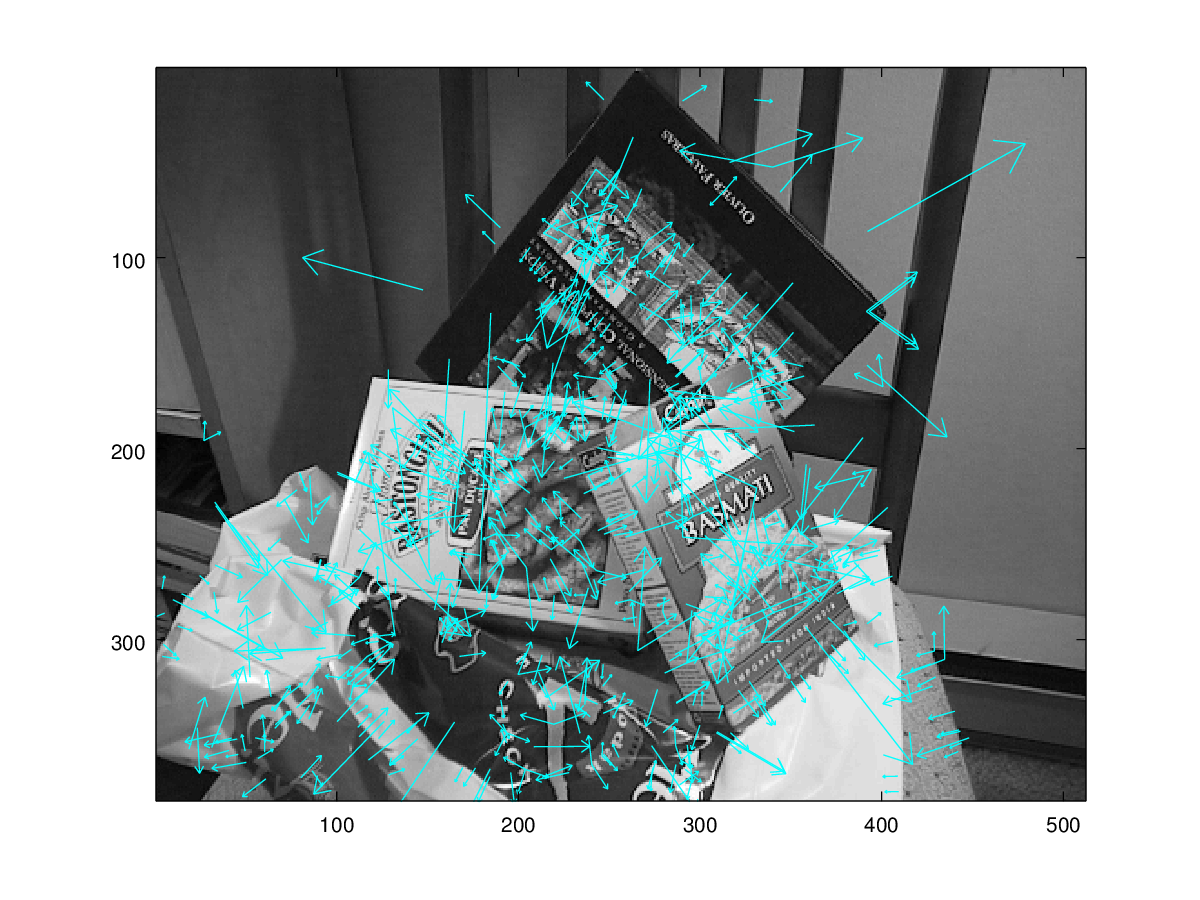
\includegraphics[width=.7\textwidth]{ex1keys}
	\label{fig:ex1keys}
	\caption{Location of the SIFT keys in scene.pgm}
\end{figure}

When matching the scene with the photo of the book cover we get 98 matches, these are shown in \autoref{fig:ex1match}. There are only two mismatches. The first is where a corner in the chair has been recognized as the corner of the book, this seems to be somewhat reasonable since they are both high contrast $90^\circ$ angle areas. The other mismatch is where a bit of the rice package got matched with one of the letters on the cover of the book. This is an odd match since there is just a random distribution of rice where the match occurs. Nevertheless, having only 2 mismatches in 98 total matches seems like a good result.

\begin{figure}[h]
	\centering
	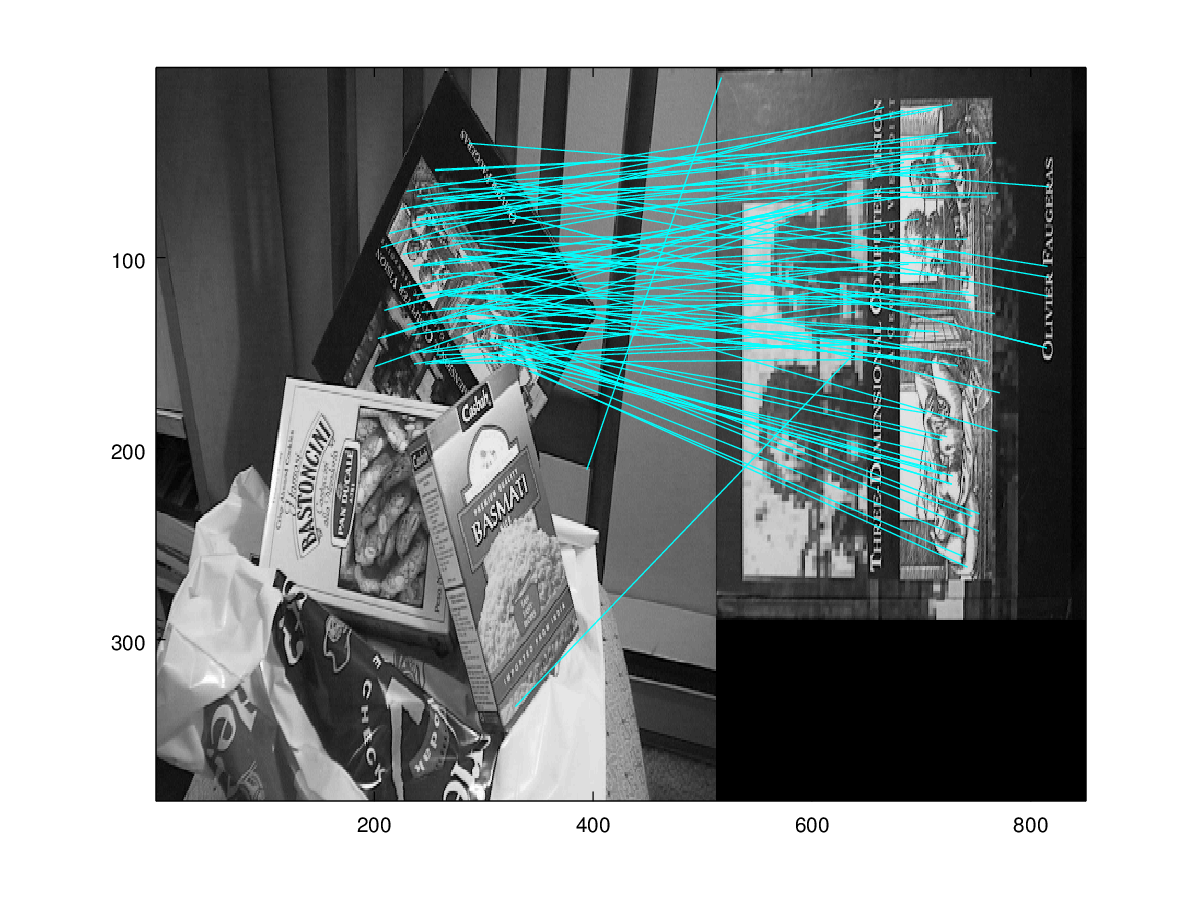
\includegraphics[width=.7\textwidth]{ex1match}
	\label{fig:ex1match}
	\caption{Matching locations in scene.pgm and book.pgm}
\end{figure}

Matching the scene with the Basmati package results in 34 matches, these are shown in \autoref{fig:ex1basmati}. There is only one mismatch in the image, this occurs on the border of the package that gets mismatched with part of the chair. Again both points in this mismatch have similar contrast.

\begin{figure}[h]
	\centering
	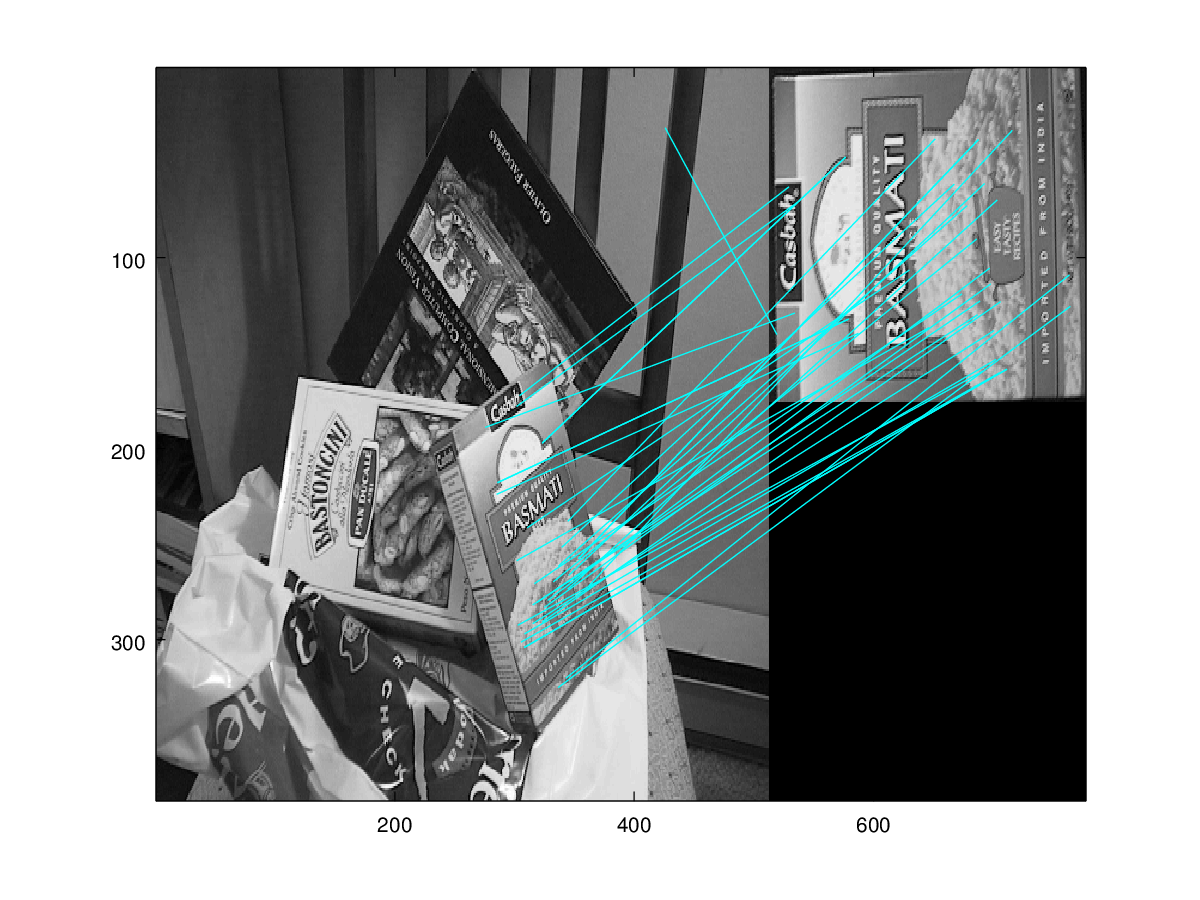
\includegraphics[width=.7\textwidth]{ex1basmati}
	\label{fig:ex1basmati}
	\caption{}
\end{figure}


\bibliographystyle{plain}
\bibliography{literature}

\end{document}